\documentclass[10pt,letterpaper,fleqn]{article}

\usepackage[utf8]{inputenc}
\usepackage[spanish,es-nodecimaldot]{babel}
\usepackage{amsmath}
\usepackage{amssymb}
\usepackage{multicol}
\usepackage{graphicx}
\usepackage{mdwlist}

\usepackage[dvipsnames]{xcolor}
\usepackage[most]{tcolorbox}

\usepackage{tabu}

\usepackage{mathtools}

\usepackage[top=1in, bottom=1in, left=1in, right=1in]{geometry}


\begin{document}

\begin{titlepage}
    \centering

    {\scshape\LARGE Universidad Nacional Autónoma de México \par}

    \vspace{1cm}
    {\scshape\Large Facultad de Ciencias\par}
    \vspace{1.5cm}

    \begin{center}
        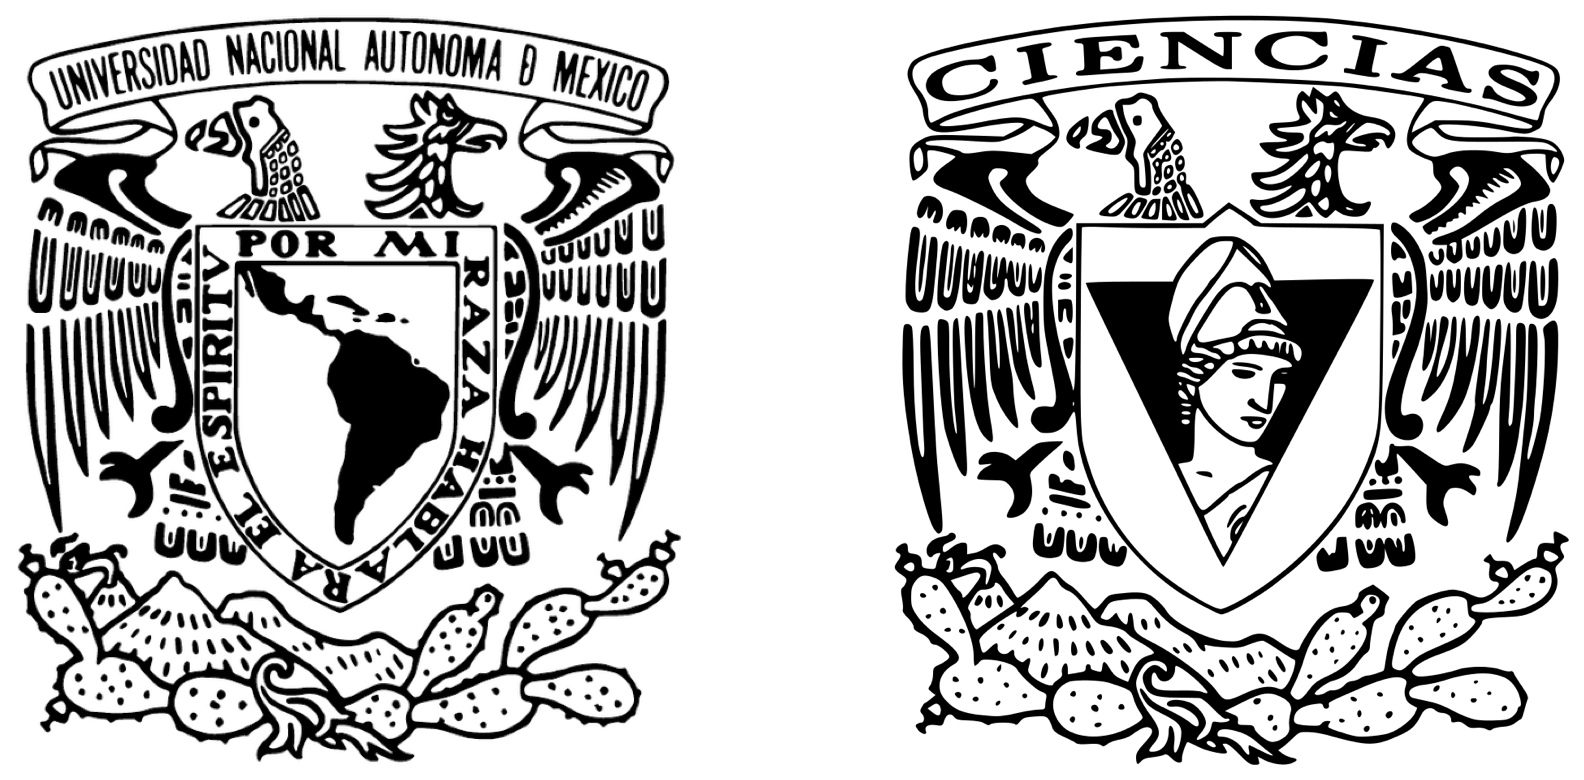
\includegraphics[scale=.1]{assets/img/logo.png}
    \end{center}

    \vspace{.8 cm}

    {\LARGE Tarea 2: \par}
    {\huge\bfseries Ejercicios \par}

    \vspace{0.5cm}
    \large{\itshape{Luis Erick Montes Garcia}} \small{ - 419004547}\\
    \large{\itshape{Hele Michelle Salazar Zaragoza}} \small{ - 316068895}


    \vfill

    Trabajo presentado como parte del curso de
    \textbf{Matematicas Aplicadas para las Ciencias II}
    impartido por el profesor \textbf{Juan Carlos Balleza}. \par
    \vspace{0.1cm}
    {\large Entrega 3 de Abril 2019 \par}
    \footnotesize{\textbf{Link al código fuente:} git@github.com:lemg98/Matematicas-Aplicadas-II.git}
\end{titlepage}

    \begin{enumerate}
        %Ejercicio 1.
        \item Sea la función vectorial $r(\overrightarrow{t}) = \left(\frac{t}{t+1},\frac{1}{t}\right)$. A continuación responda lo siguiente:
        \begin{itemize}
        	\item Calcule el siguiente límite: $$ lim_{t\rightarrow -1}r(\overrightarrow{t})$$
        	\textbf{Solución:} Observamos que al acercarnos a -1 por la izquierda $t+1$ se hace pequeño negativamente, por tanto 
        	$\frac{t}{t+1}$ tiende a infinito de manera negativa, análogamente sucede cuando nos acercamos a -1 por la derecha, este
        	tiende a infinito positivamente. Por tanto no existe el límite en ese punto


        	\item Calcule el siguiente límite: $$ lim_{t\rightarrow 0}r(\overrightarrow{t})$$
        	\textbf{Solución:} Sucede de la misma manera con este límite. Si tiende a 0 por la izquierda $\frac{1}{t}$ tiende a infinito
        	negativamente. Análogamente cuando tiende por la derecha esto tiende a infinito.

        	\item ¿Para qué valores de $t$ es discontinua la función $r(\overrightarrow{t})$? Explique su resultado.\\
        	\textbf{Solución:} Como ya mencionamos en los dos puntos anteriores no existe el límite, en los demás la función
        	es continua. Por tanto en los puntos 0 y -1 la función es discontinua.

        	\item Obtenga y dibuje los vectores velocidad y aceleración, en el punto donde $t = -\frac{1}{2}$.\\
        	\textbf{Solución:} Encontramos la primera derivada y valuamos
        	\begin{equation*}
        	\begin{split}
        		r'(\overrightarrow{t}) &= \left(\left(\frac{t}{t+1}\right)',(\frac{1}{t})'\right) \\
        							   &= \left(\frac{1(t+1) - 1(t)}{(t+1)^2},-\frac{1}{t^2}\right) \\
        							   &= \left(\frac{1}{(t+1)^2},-\frac{1}{t^2}\right) \\
				r'(\overrightarrow{-\frac{1}{2}}) &= \left(\frac{1}{(-\frac{1}{2}+1)^2},-\frac{1}{(\frac{1}{2})^2}\right) \\        							   &= \left(4,-4\right)
        	\end{split}
        	\end{equation*}

        	Encontramos ahora la segunda derivada y valuamos
        	\begin{equation*}
        	\begin{split}
        		r''(\overrightarrow{t}) &= \left(\left(\frac{1}{(t+1)^2}\right)',-\left(\frac{1}{t^2}\right)'\right) \\
        								&= \left(-\frac{2(t+1)}{(t+1)^4},-\left(\frac{1}{t^2}\right)'\right) \\
        								&= \left(-\frac{2}{(t+1)^3},\frac{1}{t^4}\right) \\
        		r''(\overrightarrow{-\frac{1}{2}}) &= \left(-\frac{2}{(-\frac{1}{2}+1)^3},\frac{1}{(-\frac{1}{2})^4}\right) \\
        								&= \left(-\frac{2}{(-\frac{1}{2}+1)^3},\frac{1}{(-\frac{1}{2})^4}\right) \\
        								&= \left(-16,16\right) \\
        	\end{split}
        	\end{equation*}


        \end{itemize}

        %Ejercicio 2.
        \item Sea la función vectorial $r (\overrightarrow{t}) = (4cos({t \over 2}),4sin({t \over 2}))$, donde $t \in [0,2\pi]$. A continuación responda lo siguiente:
        %Incisos del ejercicio 2.
        \begin{enumerate}
            %Inciso a
            \item Calcule los vectores de velocidad y aceleración.
            \\ Obtenemos la derivada de la función  $r (\overrightarrow{t})$ para obtener la {\bf velocidad}: 
            \begin{center}
                $r'(\overrightarrow{t}) = (-2sin({t \over 2}),2cos({t \over 2}))$ 
            \end{center}

            Obtenemos la derivada de la función $r'(\overrightarrow{t})$ para obtener la {\bf aceleración}:
            \begin{center}
                $r''(\overrightarrow{t}) = (-cos({t \over 2}),-\sin({t \over 2}))$ \\
                \begin{tabular}{|c|c|c|} \hline 
                    t & velocidad & aceleración \\ \hline
                    $0$ & $(0,2) $ & $(-1,0)$  \\ \hline
                    $2\pi$ & $(-0.109,1.99)$ & $(-0.99,-0.054)$  \\ \hline
                \end{tabular}
            \end{center}

            %Inciso b
            \item Grafique la función vectorial, en el intervalo de $t$ indicado.
            \begin{center}
                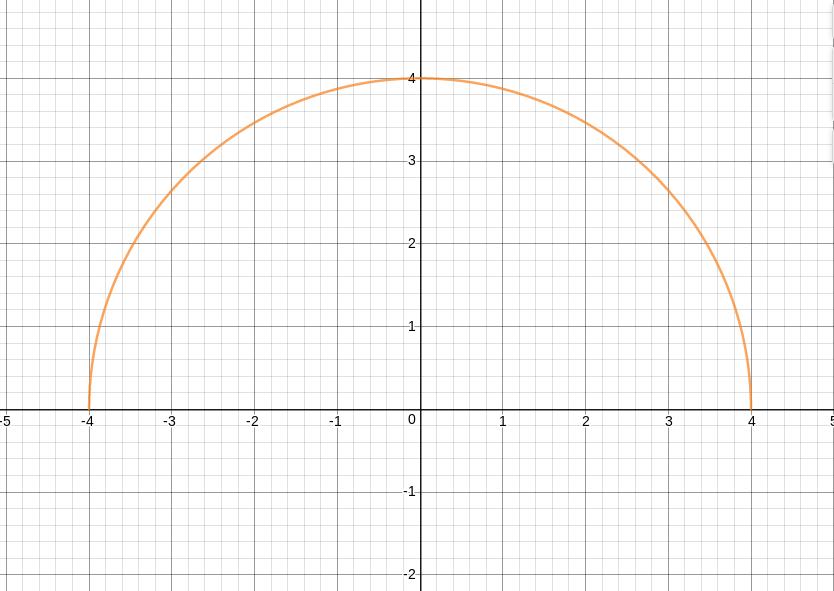
\includegraphics[scale=.3]{assets/img/ejercicio2(b).png}
            \end{center}
            %Inciso c
            \item En la gráfica de la función vectorial (inciso anterior), agregue los vectores de velocidad y aceleración en el instante $t = \pi$ 
            \begin{center}
                \begin{tabular}{|c|c|c|} \hline 
                    t & velocidad & aceleración \\ \hline
                    $\pi$ & $(-0.054,1.99) $ & $(-0.99,-0.02)$  \\ \hline
                \end{tabular}
                \\
                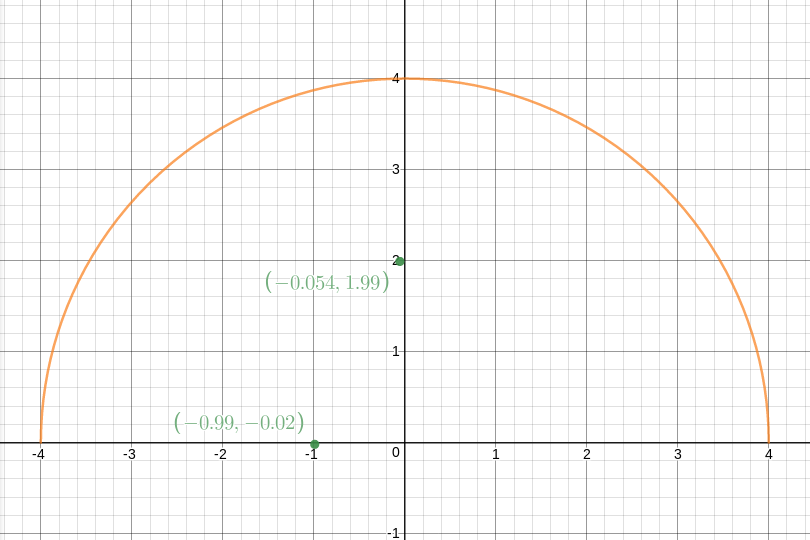
\includegraphics[scale=.3]{assets/img/ejercicio2(c).png}
            \end{center}

            %Inciso d
            \item Obtenga el ángulo entre los vectores velocidad y aceleración.
            \\ Decimos que el vector de velocidad es el vector $\overrightarrow{a}$ y que el vector de aceleración es $\overrightarrow{b}$. Para obtener el ángulo $\theta$ formamos un triángulo, siendo $\overrightarrow{a}-\overrightarrow{b}$ el lado opuesto al ángulo.
            \\ Aplicando ley de cosenos, tenemos que: \\
            $$(\overrightarrow{a} \cdot \overrightarrow{b})=||\overrightarrow{a}|| ||\overrightarrow{b}|| \cos \theta $$ \\
            Despejamos $\cos \theta$: \\
            $$\cos \theta = {(\overrightarrow{a} \cdot \overrightarrow{b}) \over ||\overrightarrow{a}|| ||\overrightarrow{b}||}$$ \\ 
            Sustituímos: \\
            $$\cos \theta = {((-0.054,1.99) \cdot (-0.99,-0.02)) \over ||(-0.054,1.99)|| ||(-0.99,-0.02)||}$$ \\
            $$\cos \theta = {((-0.054 \cdot-0.99) + (1.99 \cdot -0.02)) \over \sqrt{(-0.054)^2 + (1.99)^2} \cdot \sqrt{(-0.99)^2 + (-0.02)^2}}$$ \\
            $$\cos \theta = {0.09326 \over (1.99)(0.99)}$$ \\
            $$\cos \theta = {0.09326 \over 1.9701}$$ \\
            $$\cos \theta = {0.04733}$$ \\
            Sacamos coseno inverso: \\
            $$\theta = \cos^-1 (0.04733) = 87.29 \delta$$

        \end{enumerate}


        %Ejercicio 3.
        \item Sea la función vectorial $r(\overrightarrow{t})=(t^2, 2t-1, t^3)$. Proporcione las ecuaciones paramétricas de
        la recta que es tangente a la curva, en el punto $t_0=2$.\\
        \textbf{Solución:} Obtenemos $r(2)= (2^2,2(2) -1 , 2^3)=(4, 3, 8)$. Observamos $$r' = (2t,2,3t^2)$$, obtenemos
        $r'(2) = (2(2),2,3(2)^2) = (4,2,12)$, este es el vector de dirección. Por tanto las ecuaciones paramétricas son
        \begin{equation*}
        \begin{split}
        	x &= 4t + 4 \\
        	y &= 2t + 3 \\
        	z &= 12t + 8
        \end{split}
        \end{equation*} 

        %Ejercicio 4.
        \item Proporcione la función vectorial $r(\overrightarrow{t})$, tal que cumpla las siguientes condiciones:
        %Incisos del Ejercicio 4.
        \begin{enumerate}
            %Inciso a
            \item $a(t)=(-1,-1,-1)$ \\
            $x = y = z = -1 + 0t$ \\
            $(x,y,z)=(-1+ t0,-1+ t0,-1+ t0)$ \\
            $(x,y,z)=(-1,-1,-1)+(0t,0t,0t)$ \\
            $(x,y,z)=(-1,-1,-1)+t(0,0,0)$ \\
            $a=(-1,-1,-1)+t(0,0,0)$ 
            %Inciso b
            \item $v(0)=(0,0,0)$ \\
            $x=y=z=0$ \\
            $(x,y,z) = (0+0t,0+0t,0+0t)$ \\
            $(x,y,z) = (0,0,0)+(0t,0t,0t)$ \\
            $(x,y,z) = (0,0,0)+t(0,0,0)$ \\
            $v = (0,0,0)+t(0,0,0)$ 

            %Inciso c
            \item $r(0)=(10,10,10)$ \\
            $x=10$ ; $y=10$ ; $z=10$ \\
            $(x,y,z) = (10+0t,10+0t,10+0t)$ \\
            $(x,y,z) = (10,10,10)+(0t,0t,0t)$ \\
            $(x,y,z) = (10,10,10)+t(0,0,0)$ \\ 
            $v = (10,10,10)+t(0,0,0)$

        \end{enumerate}
(
        %Ejercicio 5.
        \item En el instante $t = 0$, una partícula se encuentra en el punto $A(1,2,3)$. Viaja siguiendo una línea recta
        hasta el punto (4,1,4) y tiene una rapidez de 2(en el punto $A$) y aceleración constante $a(t) = 3i - j + k$.
        Proporcione la ecuación del vector de posición $r(t)$ en el instante $t$.

        %Ejercicio 6.
        \item Considere la función vectorial $r(\overrightarrow{t})= ([\cos t]^3,[\sin t]^3)$. Responda lo siguiente:
        %Incisos del Ejercicio 6.
        \begin{enumerate}
            %Inciso a
            \item Obtenga el vector tangente unitario a la curva. \\
            Parametrizamos la función:
            $r(\overrightarrow{t})= ([\cos t]^3,[\sin t]^3)$ \\
            $\begin{bmatrix}
            {d \over dt} \cos^3 t \\
            {d \over dt} \sin^3 t \\
            \end{bmatrix}$ \\
            Encontramos un vector tangente: \\
            $\begin{bmatrix}
            -3sin(t)\cos^2(t) \\
            3sin^2(t)\cos(t) \\
            \end{bmatrix}$ \\
            Hacemos negativa la segunda componente para girar 90 grados en sentido de las manecillas del reloj. \\
            $\begin{bmatrix}
            3sin^2(t)\cos(t) \\
            -(-3sin(t)\cos^2(t))\\
            \end{bmatrix}$ \\
            Tenemos un vector normal, para hacerlo unitario, debemos dividir entre su magnitud, es decir, \\
            $$\sqrt{9sin^2(t)\cos^4(t)+9sin^4(t)\cos^2(t)}$$ \\
            Por lo tanto, la función para el vector unitario es el siguiente: \\
            $\begin{bmatrix}
            3sin^2(t)\cos(t) / \sqrt{9sin^2(t)\cos^4(t)+9sin^4(t)\cos^2(t)} \\
            3sin(t)\cos^2(t) / \sqrt{9sin^2(t)\cos^4(t)+9sin^4(t)\cos^2(t)}\\
            \end{bmatrix}$ \\
            %Inciso b
            \item Calcule la longitud de la curva para $t \in [0,{\pi \over 2}]$ \\
            $$\sqrt{9sin^2(t)\cos^4(t)+9sin^4(t)\cos^2(t)}$$ \\
            Sustituímos: \\
            $$\sqrt{9sin^2({\pi \over 2})\cos^4({\pi \over 2})+9sin^4({\pi \over 2})\cos^2({\pi \over 2})} - \sqrt{9sin^2(0)\cos^4(0)+9sin^4(0)\cos^2(0)} = 0 - 0 = 0 $$
        \end{enumerate}

        %Ejercicio 7.
        \item ¿Cuáles son las coordenadas $(x,y,z)$ del punto sobre la función vectorial $r(t)=(5\sen t,5\cos t, 12t)$
        que se encuentran a una distancia de $26\pi$ unidades del punto $(0,5,0)$ y en la dirección en la que crece
        la longitud del arco?\\
        \textbf{Solución:} observamos que $r(0) =(5\sen 0, 5\cos 0, 12(0)) = (0,5,0)$. A su vez $$v = (5\cos t,-5\sen t, 12)$$ 
        por tanto $$|v| = \sqrt{25\cos^2 t + 25\sen^2 t + 144} = \sqrt{25(\cos^2 t + \sen^2 t) + 144} = \sqrt{25+144} = \sqrt{169} = 13$$.
        Tenemos que $$26\pi = \int_{0}^{x}13 \text{ dt} = 13(x - 0)$$ Por ende $x = \frac{26}{13}\pi = 2\pi$. 
        Valuamos $r(2\pi) = (5\sen (2\pi), 5\cos (2\pi), 12(2\pi)) = (0,5,24\pi)$

        %Ejercicio 8.
        \item Obtenga la ecuación del círculo osculador para la función $y=\sin x$ en el punto de coordenadas $({\pi \over 2},1)$. Proponga $r(\overrightarrow{t})$ a partir de la "parametrización trivial" de la función. Calcule lo siguiente: 
        %Incisos del Ejercicio 8.
        \begin{enumerate}
            \item $(\overrightarrow{T})$, $(\overrightarrow{N})$ y $k$.\\
            Parametrización de la función: \\
            $x(t) = t \\
             y(t) = \sin t$
        \end{enumerate}
        Haga una gráfica con la siguiente información:
        \begin{enumerate}
            \item La función $y=\sin x$ \\
            \begin{center}
                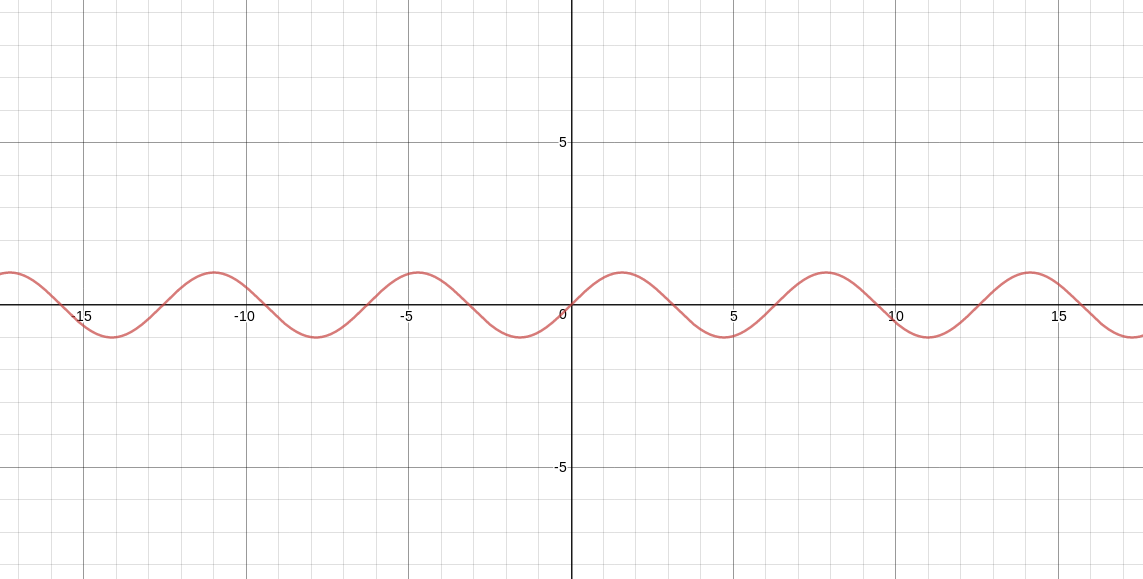
\includegraphics[scale=.3]{assets/img/ejercicio8(b).png}
            \end{center}
            \item El círculo osculador y además localizar el punto de coordenadas $({\pi \over 2},1)$
            \item Los vectores $(\overrightarrow{T})$, $(\overrightarrow{N})$.
        \end{enumerate}

        %Ejercicio 9
        \item Considere la función vectorial $r(t) = (\cos t, \sen t, -1)$
        \begin{itemize}

        	\item $r(t) = (\cos t, \sen t, -1)$
        	\item $T(t)$. Observamos $v(t) = (-\sen t,\cos t, 0)$ y $|v|= \sqrt{\cos^2 t + \sen^2 t + 0^2}=\sqrt{1} = 1$,
        		  por tanto $T(t) = (-\sen t,\cos t, 0)$.
        	\item $N(t)$. Observamos $T'(t) = (-\cos t, -\sen t, 0)$ y $|T'| = \sqrt{\cos^2 t + \sen^2 t + 0^2}=\sqrt{1} = 1$,
        		  por tanto $N(t) = (-\cos t, -\sen t, 0)$.
        	\item $B(t)$. Tenemos que $T = \textbf{k}((-\sen)^2 t - (-cos^2 t)) = \textbf{k}(\sen^2 t + \cos^2 t) = \textbf{k}$.

        \end{itemize}

        Evalue los obtenidos en (i) en el punto donde $t=\frac{-\pi}{4}$.
		\begin{itemize}
		
			\item $r(-\pi /4) = (\cos(-\pi /4), \sen(-\pi /4) , -1) = (-0.25, 0 , -1)$
			\item $T(-\pi /4) = (-\sen (-\pi /4),\cos (-\pi /4), 0) = (0, -0.25, 0)$
			\item $N(-\pi /4) = (-\cos (-\pi /4), -\sen (-\pi /4), 0) = (0.25, 0 , 0)$
			\item $B(-\pi /4) = (0,0,1)$
		\end{itemize}        


    \end{enumerate}





\end{document}